\documentclass[../../thesis.tex]{subfiles}

\begin{document}

\TODO{Introduce the section, what we think and the philosophy of presenting material in such a way.}



\section{Information theoretic/basic stats used in evaluation}

- mutual information

- entropy

- perplexity

- KL-divergence

\section{Time Series Inference}
- short-time-fourier transform etc.

\section{Neural Network}
An \textit{artificial neural network} or simply \textit{neural network} is a fundamental model in machine learning, and more specifically in \textit{deep learning}. Neural networks are loosely inspired by the way neurons are assembled in the brain. The model can be traced back the year of 1943 when Warren McCulloch and Walter Pitts developed the first artificial neuron \cite{MCCULLOCH199099}, which is considered to be the first neural model invented. It was first set out in the real world by Frank Rosenblatt in 1957 \cite{rosenblatt1957perceptron}. But not until the development of the backpropagation algorithm in its modern form in the 1980's did the model really gain traction. Neural networks have since then been the backbone in the development of machine learning, with an impressive resume of applications. Some of which, if we stretch the definition a bit, include face recognition, beating humans in chess, go and Starcraft, self-driving cars and predicting the structure of proteins. The unreasonable effectiveness of neural networks on a broad range of tasks can in part be explained by the \textit{universal approximation theorem}, proven by Kurt Hornlik in 1989 \cite{HORNIK1989359}, which roughly states that a neural network can approximate any (Borel measurable) function to any desired degree of accuracy. 

\begin{figure}
    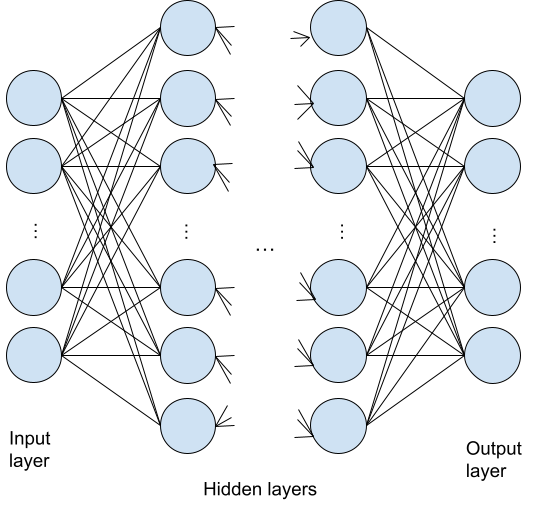
\includegraphics[scale = 0.4]{NeuralNet.png}
    \centering 
    \caption{Illustration of a Neural Network model.}
    \label{fig:NeuralNet}
\end{figure}

A neural network takes in a vector $x \in \mathbb{R}^n$ and builds a nonlinear function $f(x)$ to predict the response $y\in \mathbb{R}^m$. More specifically a neural network maps an input vector $x$ to an output vector $y$ through a series of non-linear functions of linear combinations of the input. This particular structure, presented in figure [fig of nn here] is what distinguishes neural networks from other nonlinear prediction models. The variables $x = [x_1,...,x_n]$ constitutes the units of the \textit{input layer}. The intermediate layers are called the \textit{hidden layers}, and the final mapping to $y$ is called the \textit{output layer}. A neural network is parameterized by a set of \textit{weight} matrices $W_i$ and \textit{bias} vectors $b_i$, together with a specified non-linear \textit{activation function} $\sigma$. Written out a $K$ layered neural network is given by 
\[ 
f(x) = f_K \circ f_{K-1} \circ \ldots \circ f_2 \circ f_1(x),
\]
where 
$$f_i(x) = \sigma(W_ix+b_i), \quad i \in \{1,...,K-1\},$$ 
and $f_K$ is the output layer, with application dependent structure.\\\\ 

The introduction of nonlinearity by the activation function is what enables the model to approximate nonlinear signals and differentiate itself from a linear regression model. Two of the most commonly used activation functions are $\text{Sigmoid}(x) = \tfrac{1}{1+\exp(-x)}$ and $\text{ReLU}(x) = \max(0,x)$, but countless options exists.\newline
The architecture of neural networks, and most specializations thereof, is sequential in nature. They can effectively be described as compositions of some combination of a flavour of matrix multiplication, non-linear transformation and down or upsampling. 

\subsection{Training Neural Networks}

The training of a neural network is the process of finding values for the weight and bias parameters. The general idea governing neural network training is to optimize the parameters based on some distance metric between the predicted values and the target values. This distance metric is referred to as the \textit{loss function}, and common examples of loss functions include mean squared error (MSE) and mean absolute error (MAE). Gradient based methods, such as backpropagation, are usually used to estimate the parameters based on the loss.\newline

The backpropagation algorithm is an efficient application of the Leibniz chain rule for differentiation.\newline


For a through introduction to the subject of neural networks and the training thereof we refer to chapter 6 and 8 of \cite{deeplearningbook}.


\section{Convolutional Neural Network}
This section draws heavily on the presentation of convolutional networks in chapter 9 of \cite{deeplearningbook}.\\\\

A convolutional neural network (CNN) is a particular type of neural network that is developed to learn local features in the data. This local feature learning is enabled by the mathematical operation of convolution. In essence a CNN is a neural network where matrix multiplication is switched for convolution at least one of the layers \cite{deeplearningbook}. 

\TODO{history}
1959 visual cortex cells. The Neocognitron 1980. CNN for MNIST Yann LeCun 1989- 1998 \cite{LeCun1989ConvNet}. AlexNet: GPU training and popularization of deep neural nets.

\TODO{Why was it introduced?}
Regular neural networks have a fundamental drawback in that their computational complexity 

Fully connected neural networks suffer badly from overfitting. Vanishing gradient / exploding gradient.

What problems did it solve?

\subsection{The convolution operation}

The convolution operation is an integral transform with extensive applications. It generalizes the notion of a moving weighted average. In mathematics it is ubiquitous because of its relationship with the Fourier transform.
\\\\
Let $f$ and $g$ be real valued functions, then their convolution is defined as
\begin{equation}
    (f*g)(t) = \int_{-\infty}^{\infty} f(\tau)g(t-\tau) d\tau
\end{equation}

The mathematical nuances of the exact criteria for the above integral to exist is outside the scope of this thesis, and not particularly relevant. But if $f$ and $g$ are integrable (in the Riemann or Lebesgue sense) then the convolution exists. As a rule of thumb, the convolution of $f$ and $g$ is as "smooth" as the smoothest of $f$ and $g$. It is worth mentioning that convolution is commutative, i.e that $f*g = g*f$, which can be seen by a simple change of variables. 
\\\\ 
As is typical for integral transforms, the function $g$ is referred to as the \textit{kernel}. In the context of convolutional networks the kernel consists of learnable parameters and the function $f$ is the \textit{input}. The output is sometimes referred to as the \textit{feature map} \cite{deeplearningbook}. In machine learning we handle discrete signals, represented as multidimensional arrays. As a result we must employ a discrete variation of the convolution operation. Let $I$ be the input and $K$ be the kernel, both discrete, then their convolution is defined as
\begin{equation}
    (I*K)[n] = \sum_{m=-\infty}^{\infty} I[m]K[n-m].
\end{equation}
In practice $I$ and $K$ typically has finite support, i.e they are zero for large positive and negative arguments, which circumvents any convergence problem.\\\\
Convolutions are naturally defined for higher dimensional functions, by component wise extension. For a two dimensional image $I$ and a kernel $K$ we calculate their convolution as 
\begin{equation}
    (I*K)[i,j] = \sum_{n=-\infty}^{\infty}\sum_{m=-\infty}^{\infty} I[n,m]K[i - n,j - m]. 
\end{equation}

\TODO{Figure of convolution}
\begin{figure}[h]
    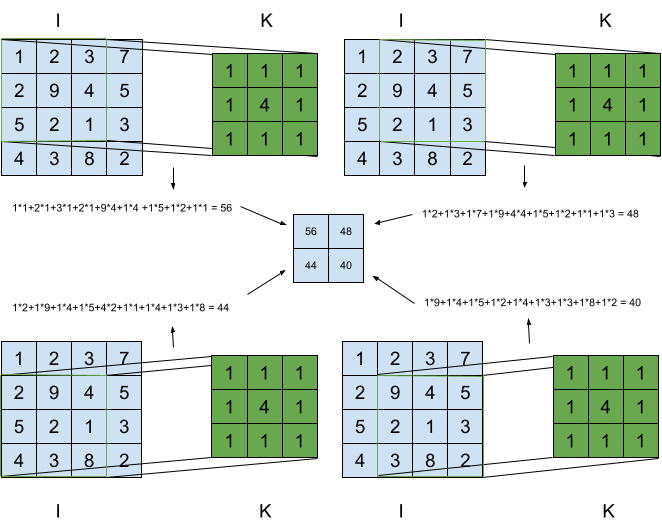
\includegraphics[scale=0.5]{Convolution.png}
    \centering    
    \caption{Illustration of discrete two dimensional convolution}
\end{figure}

- In applications the kernel dimensions are much smaller than the input dimensions. 

- Stride 

- Kernel dim and stride length determines downsample rate (reduction in size). 

- In a convolutional layer the kernel is learned such that the feature map is helpful for the training objective. 


Convolution in machine learning does not always correspond exactly to the mathematical definition of the operation, but rather to cross-correlation. The difference is just a sign flip in the kernel arguments. Operation is no longer commutative, but in practice this does not affect anything as the learned kernel parameters will be equivalent \cite{deeplearningbook}. Machine learning applications are focused on what works, rather than writing proofs. \\\\



"Convolution leverages three important ideas that can help improve ML systems: sparse interactions, parameter sharing and equivariant representations" \cite{deeplearningbook}.

\subsection{Pooling}
A pooling operation is applied as a down sample technique on feature maps in CNNs, replacing regions of the output with summary statistics. Two of the most common are max and average pooling, which replaces the region by its maximal or average value respectively. There are two hyperparameters for any pooling operation, the filter size, which determines the region of values to calculate the summary statistic, and stride length, which determines how the filter moves across the feature map. 

\begin{figure}[h]
    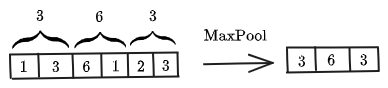
\includegraphics[scale=0.5]{MP_stride2}
    \centering    
    \caption{Max pooling of one dimensional array. Filter size: $2$, stride: $2$.}
\end{figure}
\begin{figure}[h]
    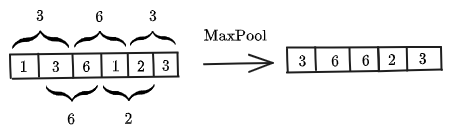
\includegraphics[scale=0.5]{MP_stride1}
    \centering    
    \caption{Max pooling of one dimensional array. Filter size: $2$, stride: $1$.}
\end{figure}

- Pooling assist in making the representations approximately invariant to small distortions of input. 

- Pooling is often essential in handling variable input size.

- 

\subsection{Architecture}
A typical layer in a convolutional network consists of three stages: 

Convolution: Hidden layer with regular matrix multiplication with weight matrix $W$ is switched out with convolution with kernel matrix $K$.

non-linear activation: Point wise nonlinearity, ReLU, sigmoid etc.

pooling layer: Max, average etc. pooling of feature map.





\subsection{Transposed Convolutional Networks}
Transposed convolution, also known as fractionally-strided convolution is a technique used to reverse the downsampling from convolutions. 




% \section{Residual Neural Network}

% Deep neural networks are hard to train. But we want deeper networks as the representations learned in deeper networks tend to be higher level/more abstract \cite{zeiler2013visualizing}. 

% The problem of exploding/vanishing gradients \todo{write about and explain what this is} has been to a large extent been solved by normalized initialization and intermediate normalization layers. This has enabled networks of tens of layers to start converging for SDG with backprop \cite{he2015deep}. \TODO{Rewrite the above in more of my own words}.



% The degeneration problem: 

% The deep residual learning framework was developed to address the degeneration problem.

% \cite{he2015deep}

% \section{Dimension reduction/visualization techniques}

% \subsection{PCA}
% Principle component analysis i a linear dimmension reduction technique which provides the axes of a point cloud 
%  PCA provides a linear projection on the eigenspace of the covariance matrix of the data. 



% \subsection{t-SNE}
% \cite{t-SNE}
% T distributed stochastic neighnourhood encoding.

% \subsection{UMAP}
% \cite{mcinnes2020umap}

% \subsubsection{densMAP}


\section{Representation Learning}

\TODO{Speak on the evaluation metrics for rep learning and the like from \cite{nozawa2022empirical}}
\cite{Rep-rev-persp}
\TODO{Sneak in something about Gödel and Turing in terms of representation. There are many philosophical aspects of this}

\subsection{What is representation learning?}
Representation learning is a term not too easily defined, one reason being the abstraction level. It is helpfull to first consider what is meant by \textit{representation} of information. Lets begin by walking through a familiar and illustrative example. Consider the base ten integer $(4)_{10} = 4$. The number can equivalently (in terms of information content) be expressed, that is represented, in any other base. The particular base we choose depends on our intention with the number. If we want to work with digital electronics, a binary representation ($(4)_{2} = 10$) is very useful, as transistors has two states. When humans do arithmetic, base ten representations of the integers are very natural, as we have ten fingers. A particular representation of information can make a task easier or harder. The information content is unchanged by a change of representation. What is changed is the easiness or difficulty of certain information processing tasks. Representation learning is then the process of learning a certain representation of information. \\\\

Representations are too highly dependent on who, or what, that will process it. An example is time. Humans have developed a standardized system for writing timestamps which works fairly well for us. But, if we want to model time dependent phenomena, say using tabular data, the DateTime representation is of very little help to a tree based model for instance. The reason being that the numerical representation of timestamps close in time is not necessarily close in numerical value. Think of 23:59 to 00:00. A possible solution is to change the representation such that the numerical values actually respect the periodic nature by mapping to the circle. The new representation is then useless for humans, but quite a lot more useful to a computer. \\\\

Anyone who has worked with data science or machine learning has come across feature engineering, and the effect good feature engineering has on a models performance. The same people too knows the level of domain expertise, creativity and time is needed to feature engineer well. One of the intriguing and promising features of neural networks, with its many specializations and architectures, is the ability to learn abstract representations of the data. This is sometimes referred to as automatic feature engineering. \todo{Find som references on higher order features learned in CNNs} In a $N$-layered network $f = f_N\circ ...\circ f_1$, the intermediate value of the data $x$ in some layer $n$, $f_n$, is what is meant by the networks learned feature representations. When we are interested in the representations learned it is helpful to dissect a model $f$, notation wise, into a \textit{feature extractor} $h$ and an \textit{output function} \todo{better name??} $g$ such that it can be factored as $f = g \circ h$. Representation learning algorithms typically follow the pattern
\begin{itemize}
    \item Train $f= g \circ h$ on some task, be it supervised, unsupervised etc.
    \item Discard $g$
    \item Use the learned feature extractor $\widehat{h}$ as part of a new model. 
\end{itemize}


The different use cases of $\widehat{h}$ is as stand alone one/few-shot learners (downstream task / frozen protocol) or as initialization of other models (pre-trained / fine-tuning protocol). \newline

When training a neural network of any variation in a supervised fashion, one always get a feature extractor, at no additional cost.  
Unsupervised representation learning loss: reconstruction in AE type, similarity losses in joint embedding networks
\TODO{When mentioning autoencoders, it is a natural spot to talk about compression. "If you can still reconstruct the signal, then you know everything about it in a sense"}


Typically in representation learning algorithms, the output dimension of $\widehat{h}$ is smaller than the input dimension. The idea of compression in representation learning has gotten theoretical and philosophical attention \todo{Information bottleneck, compression}. 


% In more general terms a \textit{feature extractor} is a mapping $h:\mathbb{R}^I \to \mathbb{R}^d$, where $I$ is the input dimension of the model. Typically $d$ is smaller than $I$.\TODO{Something about compression and effective representations}



% In supervised representation learning, the feature extractor $h$ by solving a supervised task.  Examples include $h(x) = f_n\circ ...\circ f_1(x)$ in a NN or CNN.

% One of the advantages of supervised representation learning is that one obtains the feature extractor as a byproduct of supervised learning. 
% \\\\

% Unsupervised, or self-supervised representation learning. The difference form supervised representation learning is that the feature extractor $h$ is learned by an unsupervised objective. 

% Encoder 

\subsection{Why do we care about representation learning?}
\TODO{Rewrite, i have copied to much}
Representation learning is particularly interesting because it provides one way to perform unsupervised and semi-supervised learning. It promises to unlock deep learning for unlabeled datasets. Furthermore it is known that the performance of machine learning methods is heavily dependent on the choice of data representations. Therefore much of actual efforts in deploying machine learning algorithms revolves around constructing good data pipelines and data transformations that results in representations suited for the ML algorithm. Being able to automate such processes, i.e automatic feature engineering, would solve massive problems and ease the use of ML considerably. 


\subsection{What is a good representation?}
\TODO{Talk about the trend of pre-trained models, language representations, tokenization, GPT etc}
\TODO{Rewrite, i have copied to much}
For any representations extracted of a non-invertible function, a downstream task can always be designed (in principle) to based on the lost information, hence achieve arbitrarily bad performance. The concept of universally good representations is therefore ill-defined. There is no free lunch in representation learning either. One must specify a set of predefined \textit{downstream tasks}, and evaluate according to those. The goodness of a representation is determined by how easy it makes the downstream task. Intuitively the quality of the representations are also considered higher if the the representations is able to perform well on several downstream tasks. 


\subsection{How does one evaluate representations?}
As defined in \cite{jing2019selfsupervised} a \textit{pretext task} is a pre-designed task for a network to solve, where the goal is to learn representation. A downstream task is a task used to evaluate the quality of learned representations. In general the downstream task is solved in a supervised manner, using human annotated data.\newline
We let $f = g\circ h$ be a model and train it on a pretext task in order to obtain $\widehat{f} = \widehat{g}\circ \widehat{h}$. As mentioned previously, the quality of learned representations is determined by the performance of the feature extractor $\widehat{h}$ on the downstream task. The standard evaluation protocol is to train a linear head $g_D$ on top of the \textit{frozen} representations in a supervised manner and evaluate this models performance. This is to say that we train  $f_D = g_D\circ \widehat{h}$ by only updating the parameters of the linear model $g_D$, and evaluate $\widehat{f}_D$ on some test set. A common downstream task is classification, where the idea is that good and informative representations should differentiate data in such a way that it is easy to separate them. \newline

\TODO{The role of Visual inspection}



\section{Self-Supervised learning}

Self-supervised learning (SSL) has had great success in natural language processing and computer vision in recent years. 

Machine learning can be coarsely divided into two classes, supervised and unsupervised learning. 

\subsection{Supervised}
Supervised learning refers to models who learn using labeled data. That is to say for a given input $x$ we already know what the desired output $y$ is during training, and can therefore supervise (update) our models parameters by directly comparing model output and the true value. A bit more formally, for a dataset $X = \{x_i\}_{i=1}^N$ with corresponding human annotated labels $Y = \{y_i\}_{i=1}^N$, the objective of a supervised learning algorithm is to fit $f_\theta$ in such a way that the loss across the data is minimized
\begin{equation}
    \widehat{f}_\theta = \min_\theta \frac{1}{N} \sum_{i=1}^N L(f_\theta(x_i),y_i).
\end{equation}
Common approaches to supervised learning for neural networks is to calculate some distance metric between the predicted value $\widehat{y}$ and the true value $y$ and update parameters by backpropagation.\\\\
The models falling under the supervised learning category are widely deployed and has seen tremendous success. Classical statistical models, as well as support vector machines and decision tree based models are all examples of models in this learning paradigm. The main issue with supervised learning is the need for labeled data, and labeled data is in many ways scarce.

\subsection{Unsupervised}
Unsupervised learning on the other hand refers to models or algorithms who learn exclusively from unlabeled data. That is to say that the models learn intrinsic patterns in the data. Examples of unsupervised learning models are clustering methods as K-means, K Nearest Neighbor and Gaussian mixture models, dimension reduction techniques as PCA/SVD and neural network architectures such as Autoencoders. 


\TODO{Where is it used an why?}
Exploratory data analysis, data visualization, clustering

\TODO{Pros and cons of unsupervised learning}
Unlabeled data is cheap, 

\subsection{Self-supervised}
Self-supervised learning is subcategory of unsupervised learning and refers to model who use the data itself to generate a supervisory signal, rather than external labels as in supervised learning. Even as SSL is considered unsupervised learning, the learning formulation is quite similar to that of supervised learning.\newline

For a dataset $X = \{x_i\}_{i=1}^N$ with \textit{pseudo labels} $P = \{p_i\}_{i=1}^N$ the objective of a self-supervised learning algorithm is to fit $f_\theta$ in such a way that the loss across the data is minimized. In other words find 
\begin{equation}
    \widehat{f}_\theta = \min_\theta \frac{1}{N} \sum_{i=1}^N L(f_\theta(x_i),p_i).
\end{equation}

A pseudo label is an automatically generated label from the data attributes in the pretext task. In joint embedding architectures the pseudo labels are typically some \textit{augmentation} of the original data.


\TODO{Explain why we care:}

A fruitful approach to unsupervised representation learning.\\\\

Randomly initialized networks are difficult to train and requires a lot of time and computational resources. SSL has shown remarkable results when used for pre-training. That is as models for learning network parameters who capture semantics of data, without the need for labels. Pre-training networks enables foundation models, which can be trained for many different tasks in a supervised fashion, called fine-tuning, requiring a lot less resources.

\TODO{Explain where we are now:}
In recent years, especially in computer vision applications, SSL methods have shown incredible promise in representation learning. SSL methods have proven close to, and sometimes surpassing, supervised methods on downstream tasks. \TODO{Find sources backing this up.}


\TODO{What are the different flavours of SSL? }
Autoassociative SSL - Autoencoder type - Essentially try to make composition the identity despite a compression. Usually not considered SSL, but it technically is. 
Contrastive vs non-contrastive
\TODO{What are some of the issues?}

Contrastive: Collapse, where encodes produce uninformative or constant vectors. The different ways of handling collapse. How Variance-Covariance regularization (VCReg) \cite{mialon2024variance} has emerged as a minimal(??) solution. 


\subsubsection{Contrastive}
Contrastive SSL includes both positive and negative samples. The loss function of contrasitive SSL attempts to minimize the distance of positive sample pairs (+,+) and (-,-), and maximize the distance between negative sample pairs (+,-) and (-,+).\\\\

\subsubsection{Non contrastive}

Augmentations for creating different views. The role of augmentations, types etc. Augmentations across modalities. 

\subsection{Joint embedding architecture}

Joint embedding architecture: An architecture where two networks are trained to produce similar embeddings for different views of the same data. A popular joint embedding architecture is the siamese network architecture \cite{siamese}, in which the two networks share the same weights. In models with such architecture, the existence of trivial solutions, such as both networks ignoring input and produce identical constant embeddings, is a major issue. This issue is referred to as \textit{collapse} of the model.

\subsubsection{The role of projectors}



\section{Transformers}

When was it introduced, and by whom?
What lead up to its creation?
Why and where is it now widely used? 


Wiki: A deep learning architecture based on the multi-headed attention mechanism proposed in the 2017 paper "Attention is all you need".

One fo the main novelties of the architecture is not relying on recurrence, and instead solely using the attention mechanism to capture dependencies between input and output. As recurrent models are, in computational aspects, inherently sequential, there are major challenges when training as context windows, and sequence lengths become longer. 



\subsection{The attention mechanism}

\TODO{Wait for 3b1b video for context}

\begin{figure}[h]
    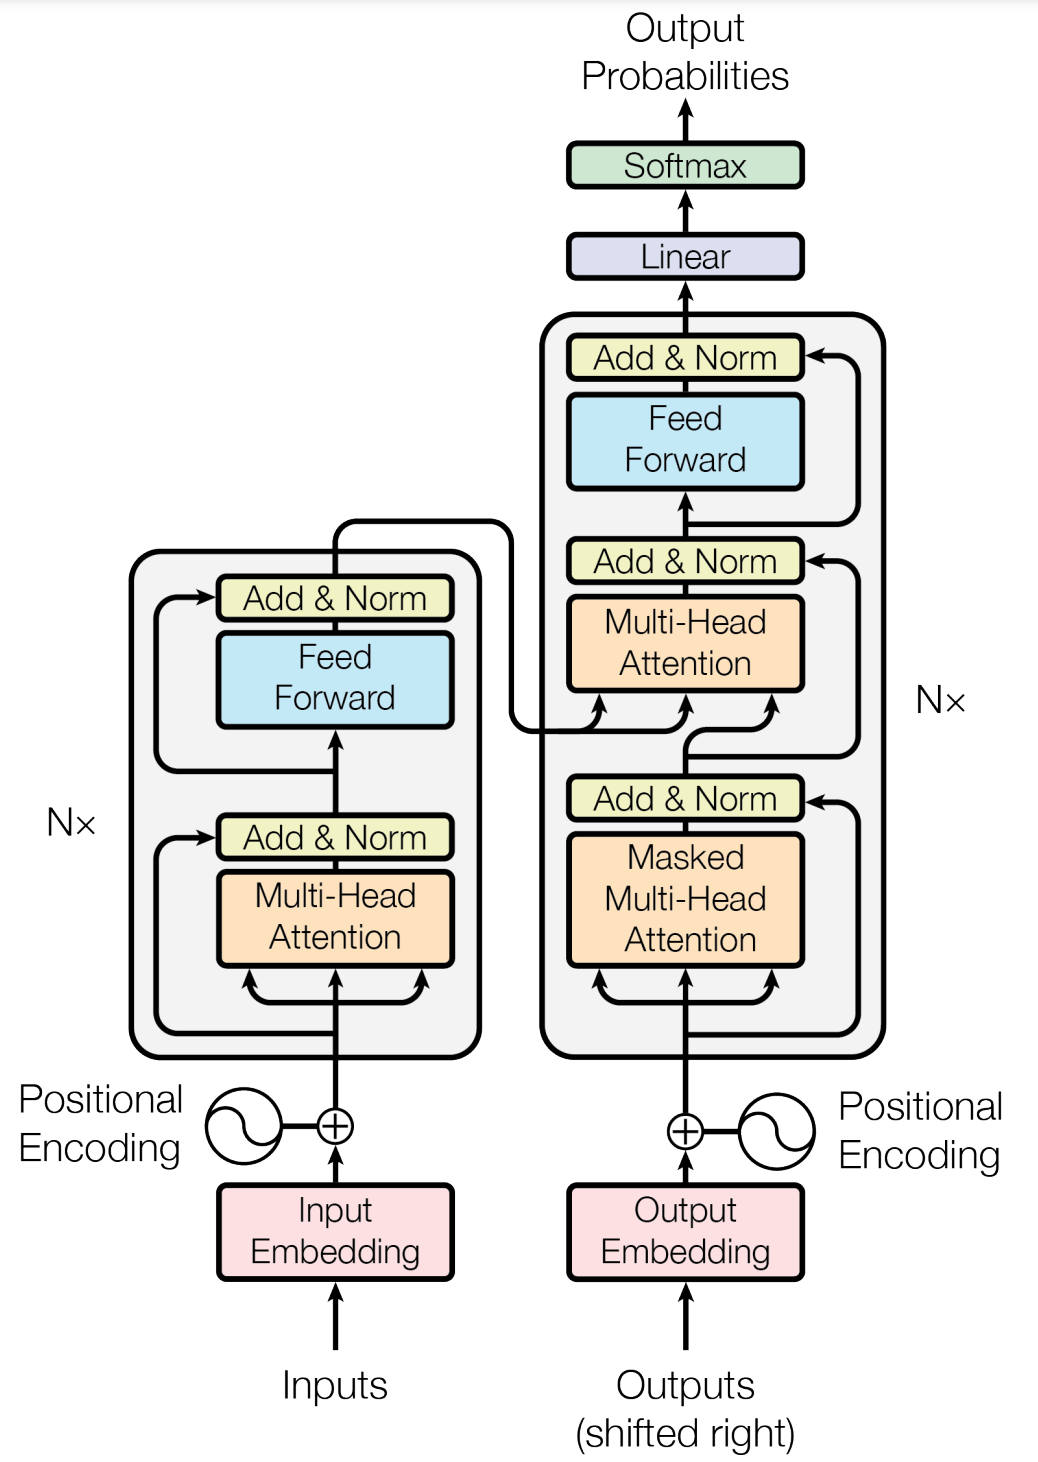
\includegraphics[scale=0.1]{Transformer_architecture}
    \centering    
\end{figure}

\subsection{Architecture}

Tokenizer

Positional encoding


Transformer layer (encoder/decoder)

\subsection{Bi-directional transformer (BERT)}

Unidirectional / 



\section{Vector Quantized Variantional Autoencoder (VQVAE)}
\subsection{Autoencoder (AE)}

\subsection{Variational Autoencoder (VAE)}
Variational Autoencoders (VAE) were introduced in \cite{kingma2022autoencoding} in 2013, and is a variational Bayes approach to approximate inference and learning with directed . 
\\\\

Let $X = \{x_i\}_{i=1}^{N}$ be a dataset of iid samples. In the VAE framework we assume that the data is a realization of some unobservable random process $Z$. This is to say that we assume there is a random variable $Z$ such that $x_i \sim p_{\theta}(x|z_i)$, where $z_i \sim p_{\theta}(z)$. As $Z$ is unobservable and the true distributions are unknown, one has to assume the form of the prior distribution $p_{\theta}(z)$ and the likelihood $p_{\theta}(x|z)$. Typically these are assumed to be Gaussian, as it allows for an array of numerical tricks to speed things up \todo{Reparameterization trick, etc, why do we use normal?}. As with any model where one wishes to employ gradient based learning, the distributions are assumed to be differentiable almost everywhere, both with respect to their parameters and argument. \\\\
VAEs have two components to their architecture. The first is an encoder, often called the inference model, $q_\phi(z|x)$ which approximates the true posterior. Secondly a decoder, often called the generative model $p_\theta(x|z)$, which approximates the likelihood. These models are typically parameterized by some type of neural network, and in that case $\phi$ and $\theta$ are the weights and biases of the two networks. 

\subsubsection{Training objective}

As with other variational methods, VAEs are optimized with respect to the \textit{evidence lower bound} or ELBO for short. Let $X$ and $Z$ be two jointly distributed variables, with distribution $p_\theta$. Then for any distribution $q_\phi$ the ELBO is defined as

\begin{equation}
    \begin{aligned}
        \label{eq:ELBO}
        \mathcal{L}_{\theta,\phi}(x) 
        &= \mathbb{E}_{q_\phi(z|x)} \log \left( \frac{p_\theta(x,z)}{q_\phi(z|x)}\right) \\ 
        &=  \mathbb{E}_{q_\phi(z|x)} \log \left( p_\theta(x)\right) + \mathbb{E}_{q_\phi(z|x)} \log \left( \frac{p_\theta(z|x)}{q_\phi(z|x)}\right) \\
        &= \log \left( p_\theta(x)\right) - \textrm{KL}(q_\phi(z|x)|| p_\theta(z|x)).
    \end{aligned}
\end{equation}

Due to the non-negativity of the KL-divergence, we see that the ELBO bounds the log likelihood of the data from below. By maximizing the ELBO with respect to the model parameters $\phi$ and $\theta$ one simultaneously maximizes the marginal likelihood, which improves the generative model, as well as reducing the KL-divergence of the approximate to the true posterior, which improves the inference model.



\begin{figure}[h]
    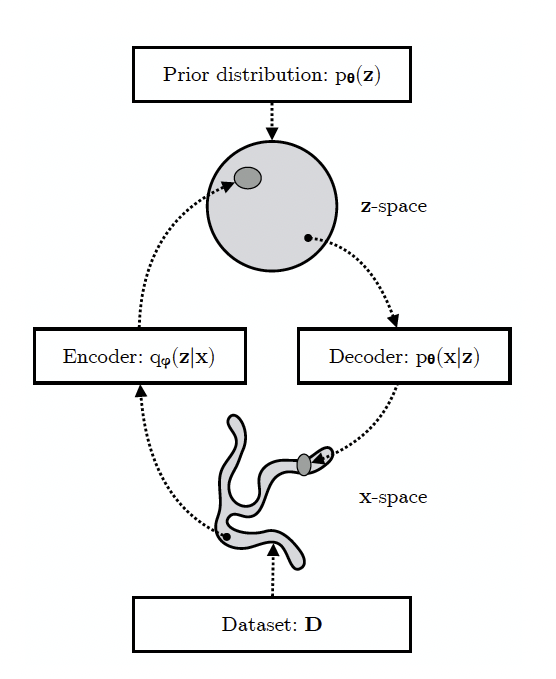
\includegraphics[scale=0.3]{VAE}
    \centering  
    \caption{\cite{VAE}, need to ask for premission or make own}  
\end{figure}

\subsection{Vector Quantization (VQ)}
Dictionary learning model

\subsection{VQVAE}
The Vector Quantized Variational AutoEncoder (VQ-VAE) was first introduced in \cite{VQVAE}. 

In contrast to VAEs, the prior and posterior is assumed to be categorical, as opposed to normal. 

Difference between VAE and VQ-VAE: 1. Maps input to discrete latent space insted of continious. 2. The prior, $p(z)$, is learned rather than static.

The posterior categorical distribution probabilities are defined as

\begin{equation}
    p(z=k | x) = 
    \begin{cases} 
        1 \quad \text{for }k = \textrm{argmin}_j||z_e(x) - e_j||_2 \\
        0 \quad \text{otherwise}
    \end{cases},
\end{equation}


\subsubsection{Loss funciton}
\begin{equation}
    \mathcal{L}_{\text{VQ-VAE}} = \mathcal{L}_{\text{VQ}} + \mathcal{L}_{\text{Recon}}
\end{equation}


VQ loss: 
\begin{equation}
    \mathcal{L}_{\text{VQ}} = ||sg(z) - z_q||_2^2 +\beta||z - sg(z_q)||_2^2
\end{equation}
     
Reconstruction loss:
\begin{equation}
    \mathcal{L}_{\text{Recon}} = ||x - \widehat{x}||_2^2
\end{equation}

How is the codebook updated? Using VQ. Ether with $l_2$ error or moving average. \\\\

Terms with stop gradient are "frozen", so the $l_2$ codebook update loss, $||sg(z) - z_q ||_2^2$ pushes the embedding vectors towards the encoder output. \TODO{Dont really onderstand why this is so. Cant seem to figure it out in the code.}

In the code quantize is x (all data) + sg(quantize - x).detatch()



Codebook loss: Distance between $z$ and $z_q$ 


\begin{figure}[h]
    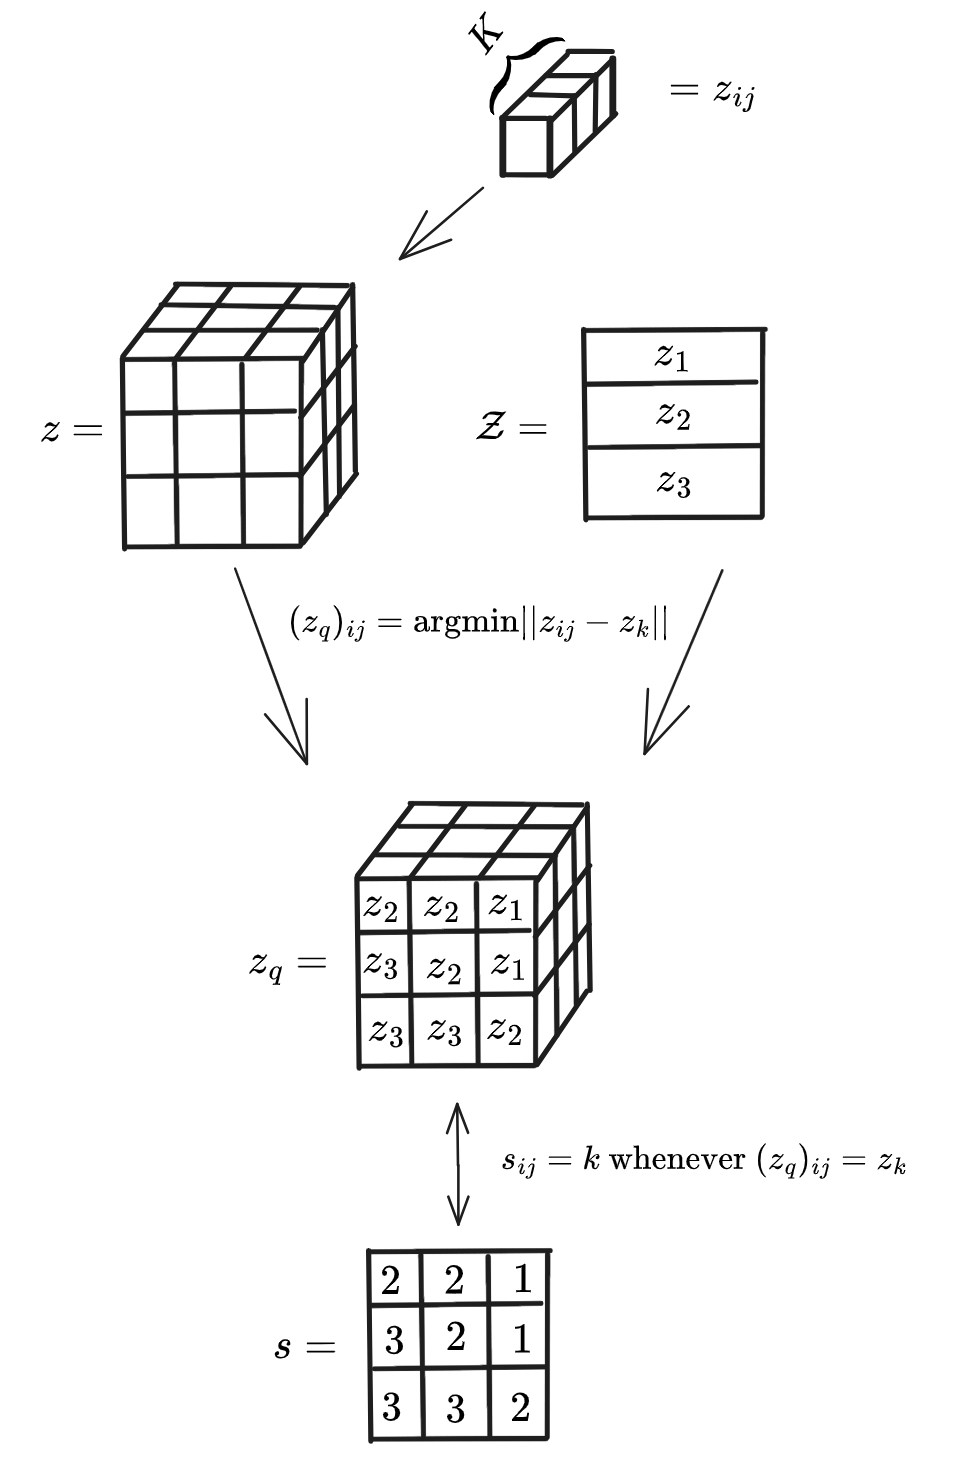
\includegraphics[scale=0.5]{quantization}
    \centering    
\end{figure}





\subsubsection{Codebook}
Vector Quantization (VQ) is a dictionary learning algorithm 

\subsubsection{Orthogonal regularization loss}
There has been several attempts to improve vector quantization. In \cite{shin2023exploration} they advocate for learning orthogonal/decorated codewords. 

% \TODO{Reference https://github.com/lucidrains/vector-quantize-pytorch some way.}


\section{Masked modelling}


\section{Evaluation metrics}

\subsection{Tokenization model}

\subsubsection{Reconstruction}

\subsubsection{Downstream Classification}




\subsection{Generative model}

\subsubsection{Visual Inspection}

\subsubsection{Inception Score (IS)}

\subsubsection{Fréchet Inception Distance (FID)}

\end{document}